% !TeX root = ../../thesis.tex
\chapter{Introduction}\label{ch:introduction}

% \instructionsintroduction

% Illustration on how to refer to your papers when using biblatex
% (see second line in thesis.tex to activate biblatex)
% \definecolor{shadecolor}{gray}{0.85}
% \begin{shaded}
% This chapter was previously published as:\\
% \fullcite{VandenBroeck2011IJCAI}
% \newpage
% \end{shaded}

In recent years the cost of generating genomic sequence data has dropped substantially.
This, coupled with improvements to the speed and usability of software packages for analyzing these data, has led to an explosion of genomic sequence availability in recent years.

\barneycomment{Put in a figure of cost of a genome vs. Moore's law as an initial motivator?}

\section{Phylogenetics}

One powerful tool at the disposal of scientists interested in inferring pathogen dynamics is that of molecular phylogenetic inference.
This is a methodology by which the shared evolutionary history of a set of genomic sequences, sometimes referred to as taxa, is hypothesized based on genomic similarity.
Phylogenetic methodologies come in many different forms, ranging from simple heuristics that approximate phylogenetic relationships based on number of observed differences between sequences\cite{felsenstein2003inferring} to highly complex models that use demographic and geographic population structure as well as state-of-the-art models of evolution to inform phylogenetic inference\cite{dudas2018mers}.
Additionally, phylogenetic analyses may be combined with other methodologies (e.g. population genetics\cite{felsenstein2003inferring} or epidemiology\cite{Black2020}) to produce robust analyses.

\newglossaryentry{mrca}{name={MRCA},description={Most recent common ancestor}}

Phylogenetic methods can help reveal many features of a set of related taxa.
The most frequent use of these methods is to construct a phylogenetic tree: a bifurcating (or sometimes multifurcating) representation of the inferred evolutionary history of a set of contemporary taxa---represented as tips or leaves of the tree---with inferred shared ancestors represented by internal nodes where two or more branches of the tree meet, eventually coalescing at the most recent common ancestor (\gls{mrca}) of all the taxa.
Such trees often use length of branches to represent genetic distance between nodes.
Often a more useful representation of evolutionary history can be found by rescaling branch lengths along a tree according to some mutation rate which provides a mapping between genetic distance and time, allowing the phylogeny to be represented as a function of time.
Phylogenetic trees can also be used to infer the shared mutation history of a set of sequences, thereby allowing the reconstruction of inferred ancestral genomes.
Similar methods may be used not only to reconstruct the ancestral states of various discrete or continuous traits that describe the taxa of the tree.
Common examples of this type of analysis include location analyses---either discrete or continuous---or analyses of a particular phenotype of interest.
Finally, phylogenetic methods often hypothesize a link between effective population sizes and tree shape---known as the coalescent process---whereby small populations are expected to have relatively high rates of branching (and therefore relatively short branch lengths) compared to larger populations.
Visual examples of all of these standard analyses are illustrated in Fig.~\ref{fig:phylogeneticsOverview}.

\begin{figure}[ht]
  \centering
  \medskip
  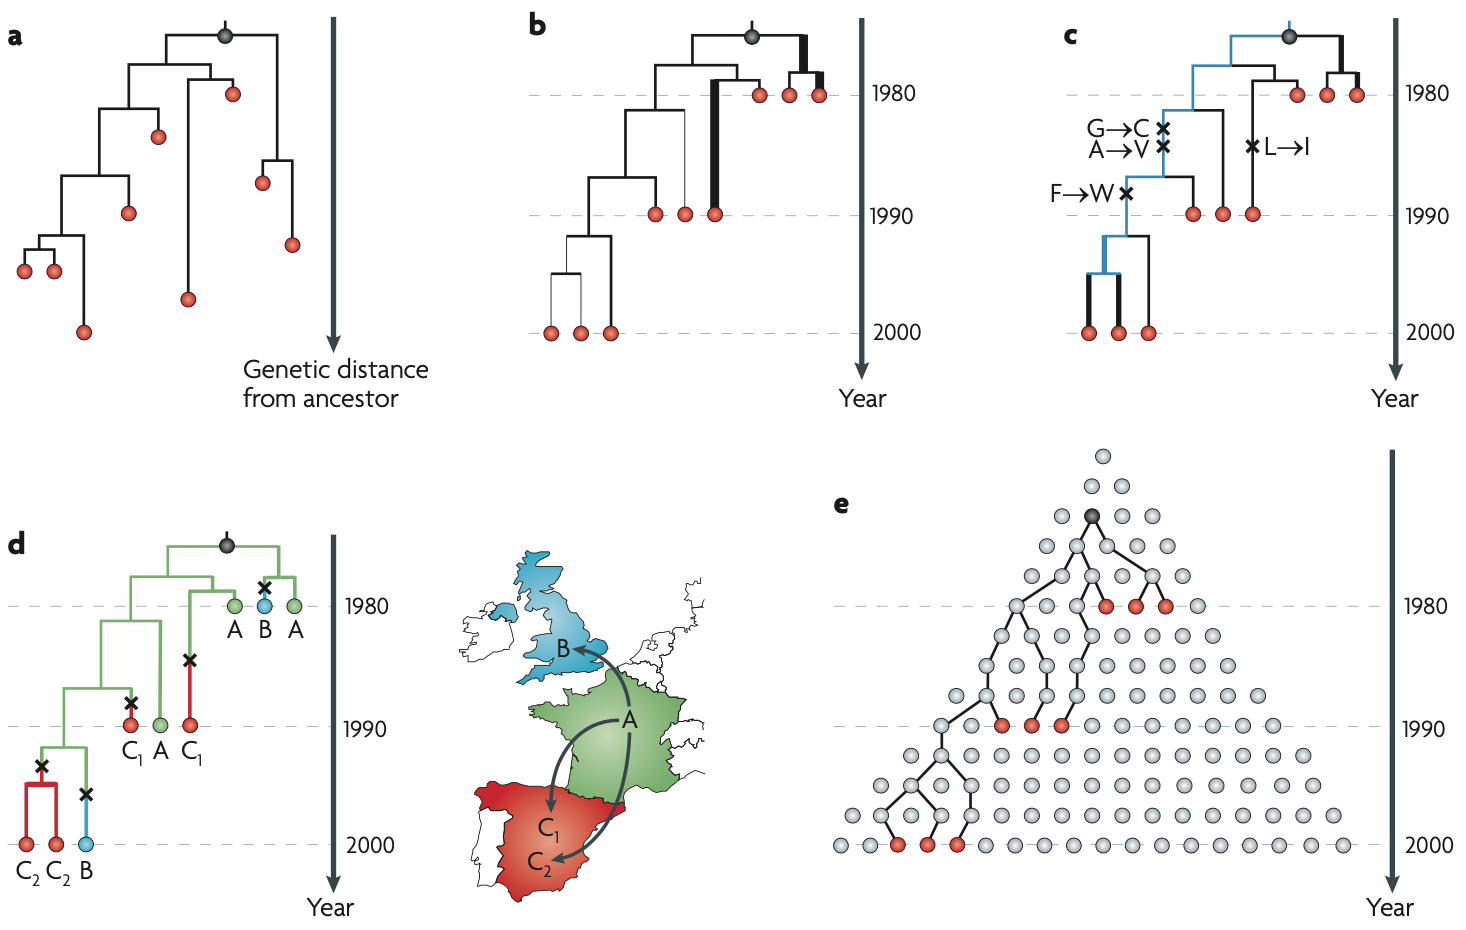
\includegraphics[width=.9\textwidth]{rambautFig}
  \caption[Applications of phylogenetic analysis]{\barneycomment{I need to write some more stuff here.}}
  \label{fig:phylogeneticsOverview}
\end{figure}

\newglossaryentry{hbv}{name={HBV},description={Hepatitis B virus}}
\newglossaryentry{lasv}{name={LASV},description={Lassa virus}}

One particularly useful application of phylogenetics is in the analysis of viral pathogen outbreaks.
Viruses represent unique study systems for both the theoretical development of phylogenetic methodologies and the implementation of phylogenetic analyses in settings with tangible public health impact.
In addition to their ubiquity and high profile within the human population, viruses prove highly suitable for phylogenetic inference because of their fast evolutionary rates, small, simple genomes, and frequent adherence to the assumptions of a single evolutionary history (i.e. infrequent recombination or reassortment).
Phylogenetic methods have frequently been used to perform \textit{post hoc} analyses of viral outbreaks, however significant work is still required before such methods can be used to inform public health responses in ``real time" during an ongoing epidemic.
In this thesis, I describe phylogenetic analyses of two viral pathogens---Hepatitis B virus (\gls{hbv}) and Lassa virus (\gls{lasv}).
We use these analyses to both illustrate both the use of current phylogenetic analysis in performing retrospective analysis, and to provide a framework for so-called ``online" phylogenetic analyses that can be performed in real-time during a viral epidemic.

\section{Bayesian phylodynamics and joint inference}

In this thesis, I devote particular to Bayesian methodologies of phylogenetic inference.
Generally, Bayesian methods are those which do not assume that the parameters which govern statistical models take a single-point value, but rather come from some posterior probability distribution.
Such methodologies are also informed by hypotheses of these parameter distributions provided \textit{a priori} by researchers---referred to as parameter priors.
Bayesian methodologies are particularly well suited to phylogenetic methods in several key ways.
Firstly, they allow researchers to create robust estimates of evolutionary histories that still account uncertainty both in the phylogenies and in other parameters of interest.
Additionally, Bayesian phylogenetic methods afford researchers the opportunity to infer many different parameters of interest (e.g. mutation rates, effective population sizes, and migration rates) jointly with the phylogeny.
Finally, these methods can be put to use with relative ease using algorithms that allow efficient exploration of posterior distributions for many parameters simultaneously.

\newglossaryentry{mcmc}{name={MCMC},description={Markov Chain Monte Carlo}}
To perform Bayesian analyses it is frequently necessary to compute very large, highly dimensional integrals to produce exact posterior distributions; this is unfortunately often infeasible to solve analytically using computers.
However, this process can be made computationally tractable by defining a Markov Chain whose stationary distribution is the desired posterior distribution of parameters.
Through this implementation, we can use Markov Chain Monte Carlo (\gls{mcmc}) methods to numerically solve for all desired parameter posterior distributions.

The implementation of such methods works according to a modified Metropolis-Hastings algorithm: first by creating a starting proposal for each parameter that is to be inferred by drawing from its prior distribution.
For numeric parameters this takes the form of one or more numbers being generated randomly, and a random tree topology is used as the initial tree.
A likelihood for the model can then be calculated, conditioned on the proposed tree and parameter set.
The candidate parameter set and tree will then be randomly permuted according to various transition kernels---referred to as ``operators"---and a new likelihood is calculated.
If the proposed parameter set yield a higher likelihood than the initial set, they are accepted as the new proposal set.
If they have a likelihood lower than the first proposal, they will be accepted with probability proportional to the ratio of their likelihoods.
This process is then repeated, until a stable parameter and tree set are found.
This stable set is considered to be the posterior distribution from which we would like to sample.
We continue to repeat the process, recording the state of the chain at regular intervals, until the posterior has been sufficiently explored.

\subsection{Measurably evolving populations and temporal signal}

While performing phylogenetic analyses, we are often interested in how populations evolve as a function of time, rather than as a function of genetic distance.
To this end, we seek a way to correlate differences in our input data (i.e. genetic distance) with time.
We do this by assuming that mutations accumulate along the branches of a phylogenetic tree according to some rate, which can be fixed to one vale across the entire phylogeny\cite{strictClockPaper}, or it can vary by branch according to sophisticated statistical models\cite{unocrrelatedRelaxedClocks, randomLocalClocks}.
We refer to this rate as a ``clock rate"---generally represented in units of substitutions per site per year.
The clock rate can be used to rescale the branches of a phylogeny from units of genetic distance to units of time.

\newglossaryentry{mep}{name={MEP},description={Measurably evolving population}}
Historically, a way that correlation has been performed is through informed estimates of divergence times between two known lineages\cite{humanApeDivergence}.
While this has proven useful for some applications, it has limited use in the inference of molecular clocks in viruses, where known divergence times may be much more limited.
Indeed, it is frequently not possible to provide accurate prior estimates of historical divergence times, and we instead wish to infer molecular clock rates directly from heterochronous (i.e. sampled over long periods of time) sequences.
We call the existence of sufficient statistical power from heterochronous sequence data to determine a molecular clock rate ``temporal signal", and we refer to a population from which we can observe a statistically significant number of mutations through time a ``measurably evolving population" (\gls{mep})\cite{drummond2003MEP}.
In general, there are two sources from which we can observe \gls{mep}s: populations with available ancient genomes, and rapidly evolving RNA viruses.
Analysis of ancient genomes has proven to be an informative way of inferring the phylodynamics of eukarytoic populations\cite{shapiro2004bison}


\subsection{Statistical and computational challenges} %GB: I would turn this into 'Statistical and computational challenges'; or perhaps leave it but make sure to explain that an important aspect to consider is acquiring sufficiently high ESS values for all relevant parameters

One of the major challenges of phylogenetic inference is the vast size of the state space of potentially inferred variables.
The size of so-called ``tree space"---the set of all possible phylogenetic trees for a given dataset---scales at the rate $\frac{(2n-3)!}{2^{n-1}(n-1)!}$.
This is far too large to exhaustively explore for the datasets that researchers are interested in; for a dataset consisting of only thirty taxa, the number of possible rooted, labeled phylogenies numbers over $10^{38}$\cite{felsenstein2003inferring}.
For the datasets that we explore in this thesis---ranging in size to 769 taxa---this number grows to vastly overshadow the number of atoms in the observable universe.
As such, exhaustively exploring this space is impossible, and traversing this space algorithmically can still take considerable time.

\subsubsection{Effective sample size and burnin}
\newglossaryentry{ess}{name={ESS},description={Effective sample size}}
Bayesian phylogenetic inference of large, complex datasets can take upwards of a month of constant compute time before a chain reaches convergence and has adequately explored the full posterior distribution.
During this time, we take ``samples" at fixed intervals by recording the state of all parameters of the chain.
We quantify how fully the posterior has been sampled using a metric known as Effective sample size (\gls{ess}).
Because sequential samples of the chain's state are frequently highly correlated, we use \gls{ess} as a metric for how many fully independent, uncorrelated sample equivalents we have accumulated.
We generally seek to accumulate \gls{ess} values over 200 for each parameter in our model. \barneycomment{why??}

A significant amount of computation time is consumed by the chain moving from where it (randomly) began in state space toward the posterior distribution---a period referred to as ``burnin".
Because the chain is rapidly traversing parameter space during this period all samples are correlated, and we are therefore unable to accumulate any \gls{ess} during this time.
Indeed, the entire burnin period is discarded prior to analysis.
The burnin period typically takes roughly 10\% of the total computation time.
A major computational issue stemming from the burnin period is that the time spent in burnin can only be mitigated by specifying prior distributions that are strongly informative of the posterior distribution.
This means that even if identically parameterized chains are run in parallel the burnin period must take place for each independent run, significantly lowering the effectiveness of chain-level parallelization.


\subsection{BEAST}

\newglossaryentry{beast}{name={BEAST},description={Bayesian Evolutionary Analysis Sampling Trees}}
For the analyses described in this thesis, we make use of the software package Bayesian Evolutionary Analysis Sampling Trees 1.10 \cite{beast} (\gls{beast}).
BEAST a flexible tool in which many Bayesian phylogenetic models---and their associated priors and transition kernels---have been implemented and optimized such that large datasets may be easily specified and run efficiently on a wide variety of compute resources.
This tool implements Bayesian phylogenetic inference via \gls{mcmc} in a way that is easy to use, and flexible.
Analyses in \gls{beast} are facilitated by hardware optimization libraries\cite{beagle}, as well as a large suite of utility programs that make running analyses in parallel and quickly interpreting results feasible.

\section{Viral pathogens}
Viral pathogen outbreaks are a particularly useful study system for Bayesian phylogeneticists because their relatively small, simple genomes rate typically facilitate tractable computation.
The rapidity with which viruses move though populations and their fast clock rates give many viral pathogens rather strong temporal signal, and therefore meke them good candidates for Bayesian phylogenetic inference.
Beyond their ease of analysis, viral pathogens make interesting study systems because of the large influence that they exert on human quality of life.
Viruses frequently cause human suffering and death, both as endemic diseases (seasonal influenza, hepatitis, etc.) and the agents behind sudden disease epidemics (Zika, Ebola, Lassa).
Indeed, viruses have been responsible for the majority of the most deadly pandemics of the last century (1918 Spanish influenza, 2009 Swine flu, COVID-19).
Even when they do not cause large-scale epidemics or global pandemics, or when they do not cause death, viruses can still cause vast amounts of human suffering though localized, small-scale outbreaks that cause severe health problems for those that they infect.
In this thesis, I present the results of Bayesian phylogenetic analyses of two separate viral pathogens: Hepatitis B virus (\gls{hbv}) and Lassa virus (\gls{lasv}).

\subsection{Hepatitis B virus}

\gls{hbv} has infected over two billion people worldwide, and puts over 350 million people at risk of cirrhosis and liver cancer \cite{kane1995}.
The virus is classified into eight different genotypes based on genomic sequence divergence.
These genotypes show strong ethnospatial patterns, and are often correlated directly to the region of the world where they are most prominent \cite{schaefer2007}.
Hepatitis B virus consists of two partially overlapping strands of DNA (Fig.~\ref{fig:hbvGenome}).
The long strand ranges from 3,020--3,320 bases in length, while the short strand ranges from 1,700--2,800 nucleotides long, depending on genotype \cite{kay2007_hepatitis_b_virus_genetic_variability}.

\begin{figure}[ht]
  \centering
  \medskip
  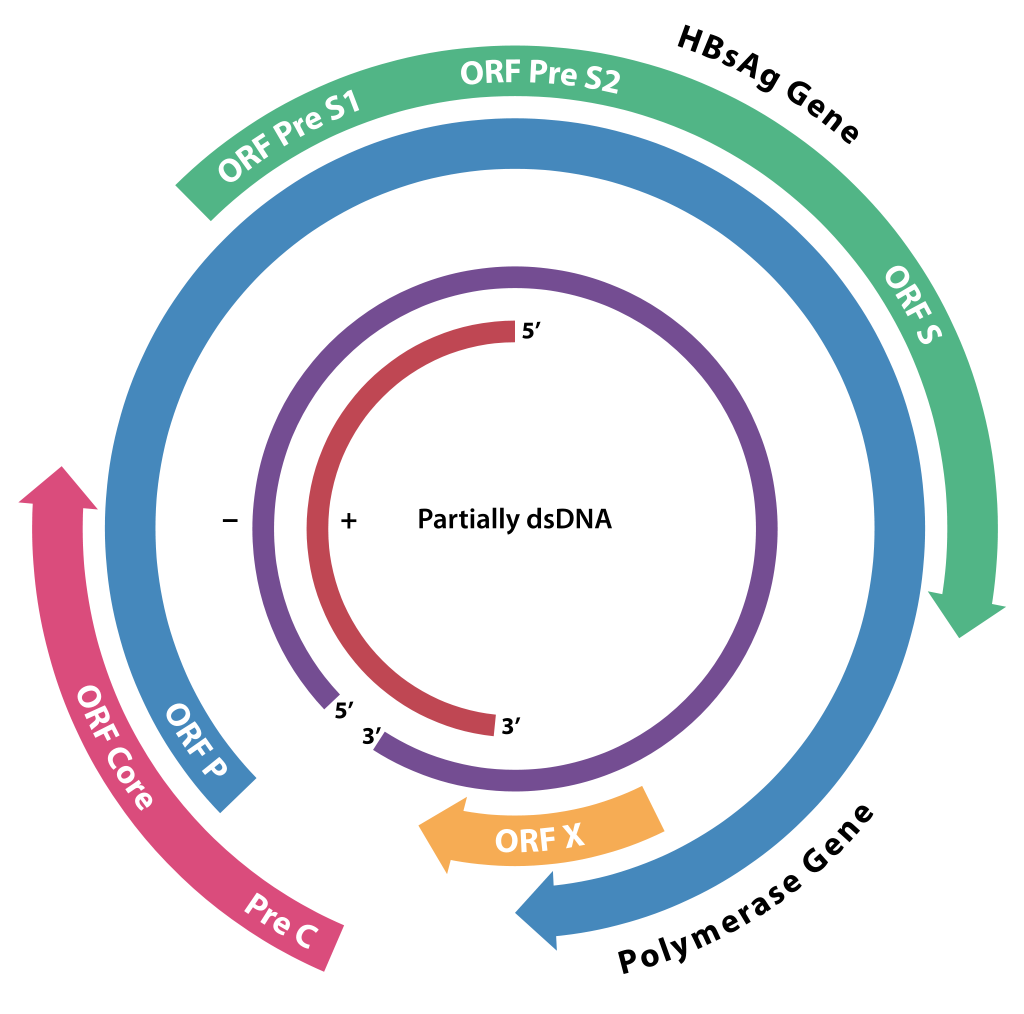
\includegraphics[width=.6\textwidth]{hbv_genome_schematic}
  \caption[Scematic of the HBV genome]{The \gls{hbv} genome consists of two partially overlapping strands of DNA. The long strand (purple) is roughly 3 kb in length and circular, while the shrot strand (red) is roughly 2.2 kb in length. Between the two strands there are four identified open reading frames. (\textit{Photo credit: Wikimedia Commons}\cite{HBVwiki})}
  \label{fig:hbvGenome}
\end{figure}

\subsection{Lassa virus}

Lassa virus (\gls{lasv}) is the causative agent of Lassa fever, a viral hemorrhagic fever that infects 300,000--500,000 people anually and causes 54,000--90,000 deaths yearly \cite{three, lassa, papers}.
\gls{lasv} has a genome that is divided into two segments: a large (L) segment approximately 7.5 kb in length, and a small (S) segment approximately 3.5 kb in length.
The L segment encodes genes \textit{Pol} and \textit{Z}, while the S segment encodes genes \textit{GPC} and \textit{NP}.

\barneycomment{Maybe include a figure from Liana's dissertaton}


%%%%%%%%%%%%%%%%%%%%%%%%%%%%%%%%%%%%%%%%%%%%%%%%%%
% Keep the following \cleardoublepage at the end of this file,
% otherwise \includeonly includes empty pages.
\cleardoublepage

% vim: tw=70 nocindent expandtab foldmethod=marker foldmarker={{{}{,}{}}}
